
\documentclass[a4paper,12pt]{article}
\usepackage[latin1]{inputenc}
\usepackage[spanish,es-nodecimaldot]{babel}
\usepackage[T1]{fontenc}
\usepackage[intlimits]{amsmath}
\usepackage{graphicx}
\usepackage{a4wide}
\usepackage{float}
\usepackage{caption}
\usepackage{subcaption}

\usepackage{tikz}
\usetikzlibrary{trees}
\usepackage{xcolor}

\graphicspath{{imagenes/}}

\title{\textsc{Modelo de Ising en 2D} \\ \vspace{2em} \Large{Introducci�n a la 
simulaci�n computacional}}
\author{\small{Luis Pizarro (lpizarro@cnea.gov.ar)} \\
        \small{Pablo Bellino (pbellino@gmail.com)}}

\date{Octubre de 2015}


\begin{document}
\maketitle

\begin{abstract}
Un resumen
\end{abstract}


\section{Introducci�n}
Empezamo


\begin{equation}{\label{eq:hamiltoniano}}
H = - J \sum_{\langle ij \rangle}^N s_is_j
\end{equation}

\noindent donde $\langle ij \rangle$ indica que la sumatoria se realiza con los 
sitios primeros vecinos.

La magnetizaci�n asociada a un dado estado se define como:

\begin{equation}
M = \mu \sum_{i=1}^N s_i
\end{equation}

Se puede demostrar que la temperatura cr�tica, expresada en unidades 
adimensionales es:

\begin{equation}
\frac{k T_c }{J} = \frac{2}{ln(1+\sqrt{(2)})}
\end{equation}

\noindent siendo $k$ la constante de Boltzman

\tikzstyle{every node}=[thick,anchor=west, 
font={\scriptsize\ttfamily}, inner sep=2.5pt]
\tikzstyle{selected}=[draw=blue,fill=blue!10]
\tikzstyle{root}=[draw=blue, fill=blue!30]

\begin{figure}[H]\label{fig:arbol.dir}
\begin{center}
\begin{tikzpicture}[%
    scale=.7,
    grow via three points={one child at (0.5,-0.65) and
    two children at (0.5,-0.65) and (0.5,-1.2)},
    edge from parent path={(\tikzparentnode.south) |- (\tikzchildnode.west)}]
  	\node [root] {bin}
  	child { node [red] {ising}}
  	child { node [red] {corridas\_paralelo.py}}
  	child { node {tablas\_temperatura.dat}}
    child { node [selected] {0.5\_tmpfolder}
      child { node {parametros.dat}}
      child { node {runs\_estadistica.dat}}
      child { node [selected] {RUN00}
	     child { node {val\_medios.dat}}
	     child { node {estado.dat}}
	     child { node {ultimo\_estado.dat}}
      }
      child { node at(0,-1.8) [selected] {RUN01}}
      child { node at(0,-1.9) [selected] {RUN02}}
      child { node at (0,-2.0) {\dots}}
    }       
    child { node at (0,-5.5) [selected]{0.6\_tmpfolder}}
    child { node at (0,-5.8)[selected] {0.7\_tmpfolder}}
    child { node at (0,-6.1) {\dots}};
\end{tikzpicture}
\end{center}
\caption{Esquema de carpetas y archivos que se obtienen al realizar una corrida 
completa haciendo estad�sticas en cada temperatura.}
\end{figure}]


%\begin{eqnarray}
%  f_r(x) &=& \frac{4}{\pi - 4}\frac{x^2}{1+x^2} \\
%  f_\theta(x) &=& \frac{\sin(x)}{2} \\
%  f_\varphi(x) &=&  \frac{1}{2\pi} 
%\end{eqnarray}

\begin{figure}
	\begin{center}
	\begin{subfigure}{.49\textwidth}
		\centering
      	\includegraphics[scale=0.4]{{terma_t0.5_ei_rand}.pdf} \\
     	 \caption{Temperatura 0.5}\label{fig:terma.t05_rand}
	\end{subfigure}
	\begin{subfigure}{.49\textwidth}
		\centering
     	 \includegraphics[scale=0.4]{{terma_t5.0_ei_up}.pdf} \\
      	\caption{Temperatura 5.0}\label{fig:terma.t50_up}
	\end{subfigure}
	\end{center}
\end{figure}

\begin{figure}
	\begin{center}
	\begin{subfigure}{.49\textwidth}
		\centering
      	\includegraphics[scale=0.4]{{terma_t3.0_ei_rand}.pdf} \\
     	 \caption{Temperatura 0.5}\label{fig:terma.t3_rand}
	\end{subfigure}
	\begin{subfigure}{.49\textwidth}
		\centering
     	 \includegraphics[scale=0.4]{{terma_t3.0_ei_up}.pdf} \\
      	\caption{Temperatura 5.0}\label{fig:terma.t3_up}
	\end{subfigure}
	\end{center}
\end{figure}

\begin{figure}[H]
    \begin{center}
      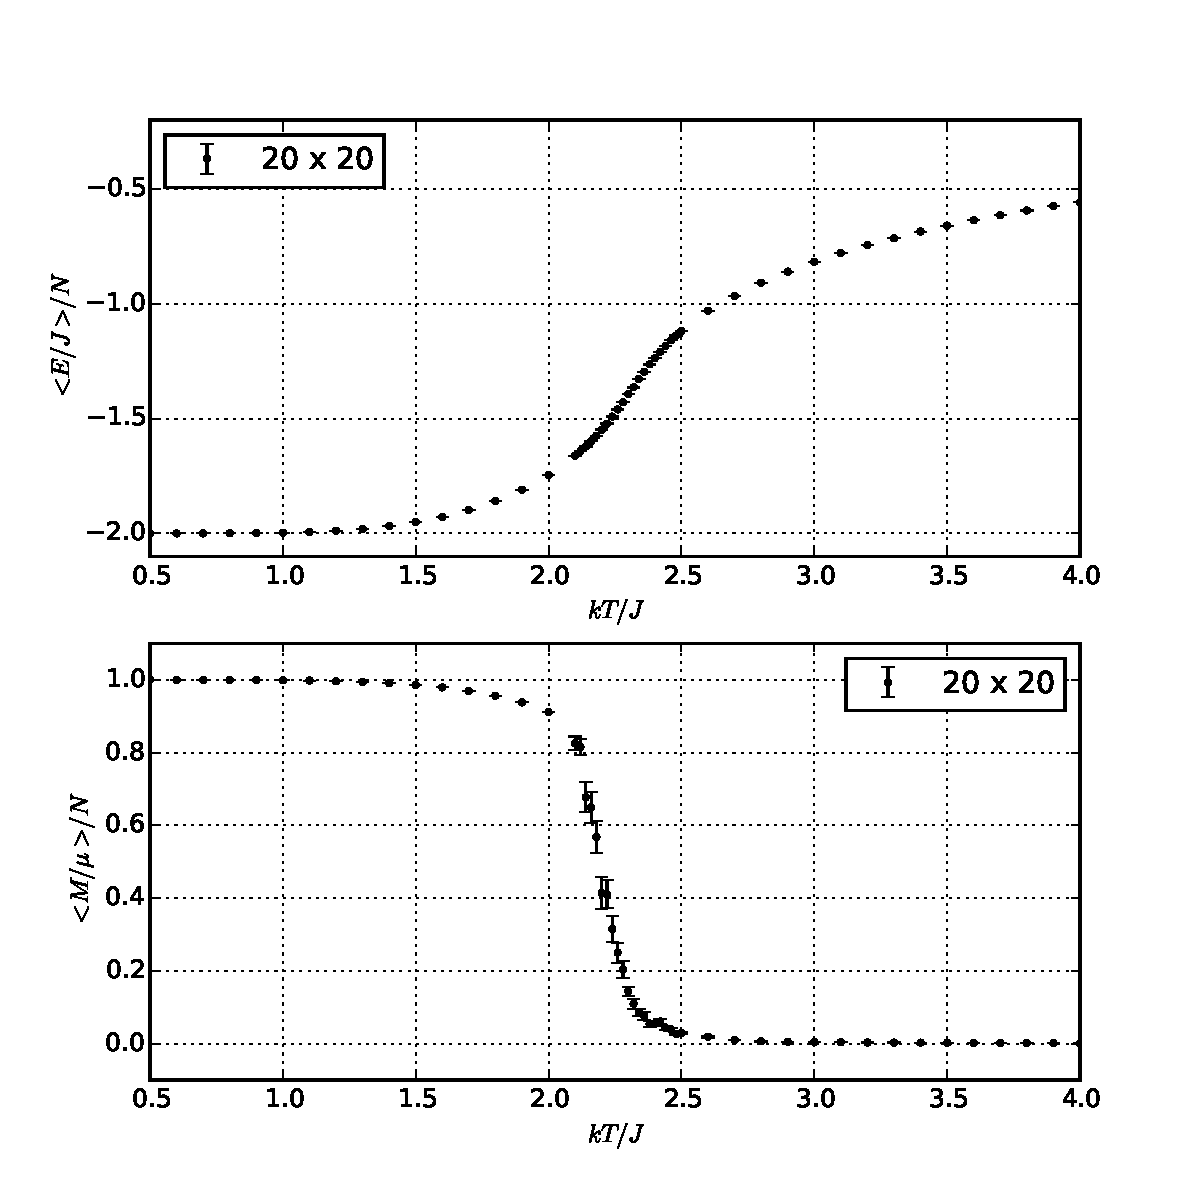
\includegraphics[scale=0.6]{val_medios.pdf} \\
      \caption{Distribuci�n poissonianas $P(4)$, $P(10)$ y $P(40)$. En rojo 
      aparecen las distribucciones gaussianas para cada 
      caso.}\label{fig:val_medios}
    \end{center}
\end{figure}


\begin{figure}[H]
    \begin{center}
      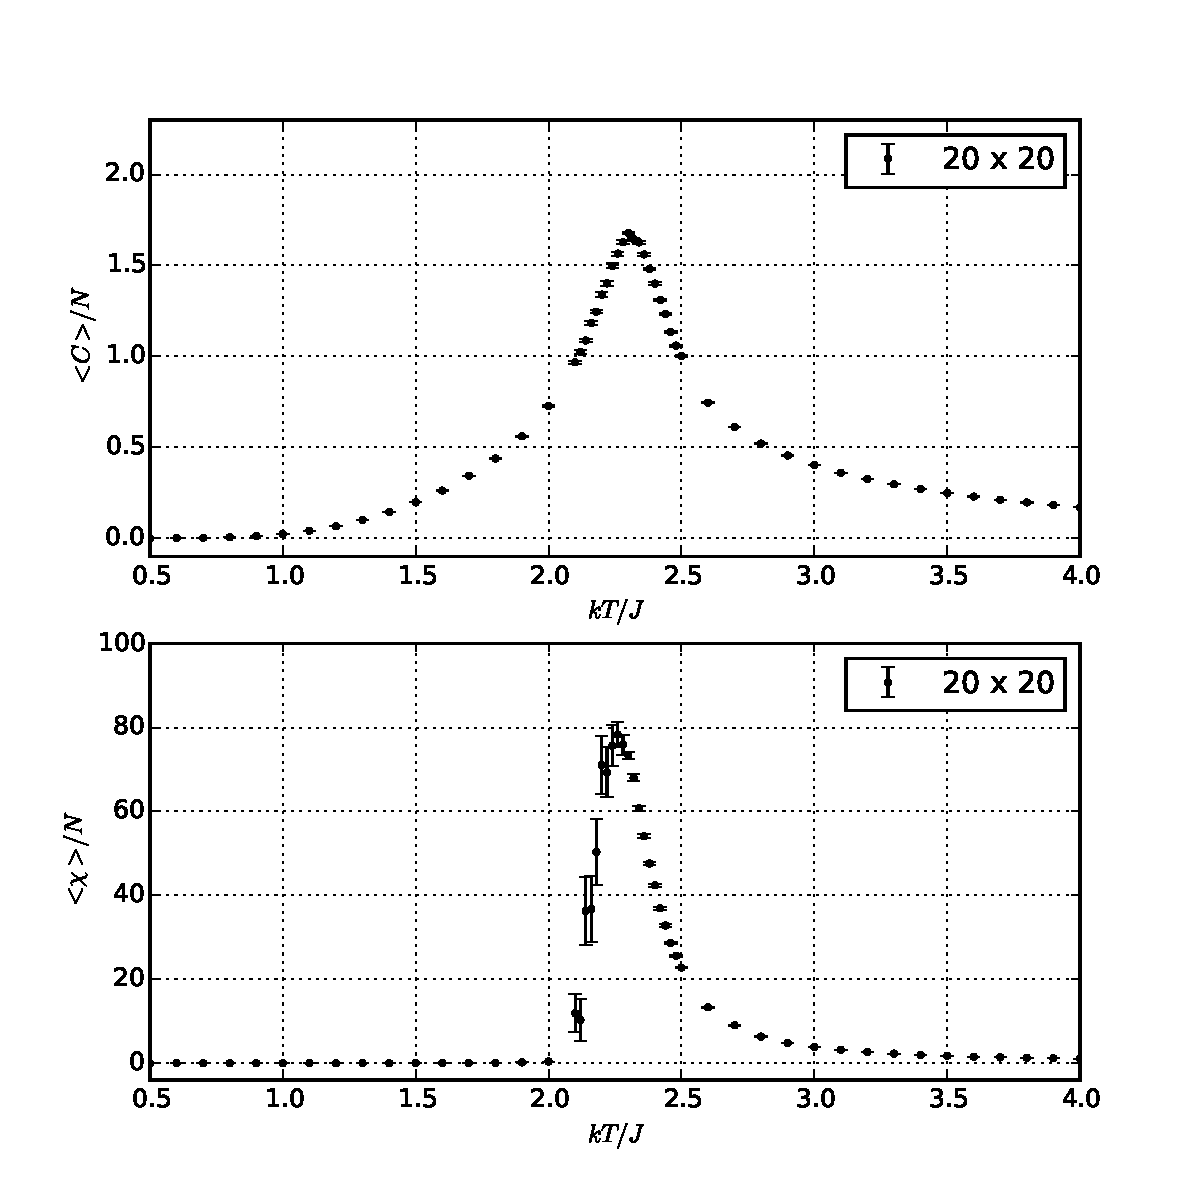
\includegraphics[scale=0.6]{fluctuaciones.pdf} \\
      \caption{Distribuci�n poissonianas $P(4)$, $P(10)$ y $P(40)$. En rojo 
      aparecen las distribucciones gaussianas para cada 
      caso.}\label{fig:fluctuaciones}
    \end{center}
\end{figure}

\begin{figure}[H]
    \begin{center}
      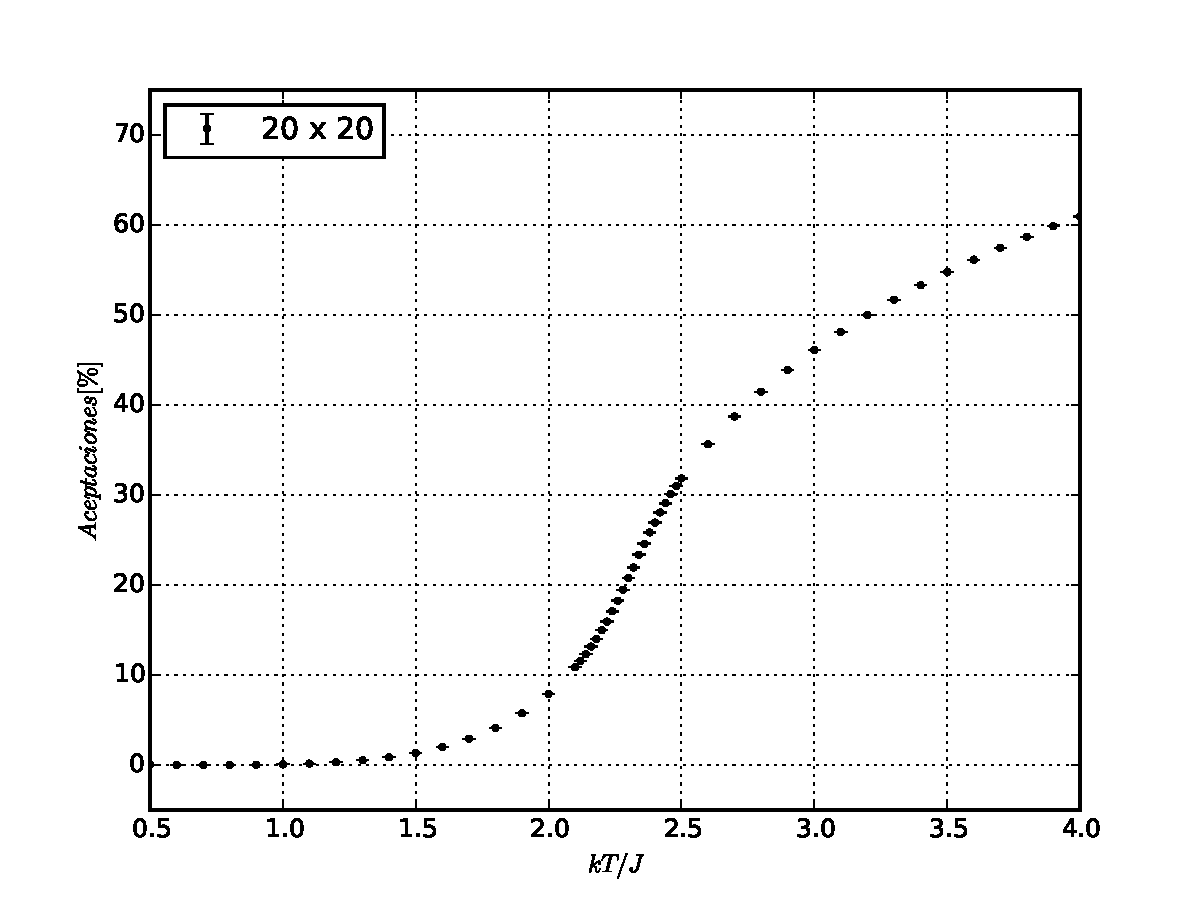
\includegraphics[scale=0.5]{aceptaciones.pdf} \\
      \caption{Distribuci�n poissonianas $P(4)$, $P(10)$ y $P(40)$. En rojo 
      aparecen las distribucciones gaussianas para cada 
      caso.}\label{fig:aceptaciones}
    \end{center}
\end{figure}


\begin{figure}[H]
    \begin{center}
      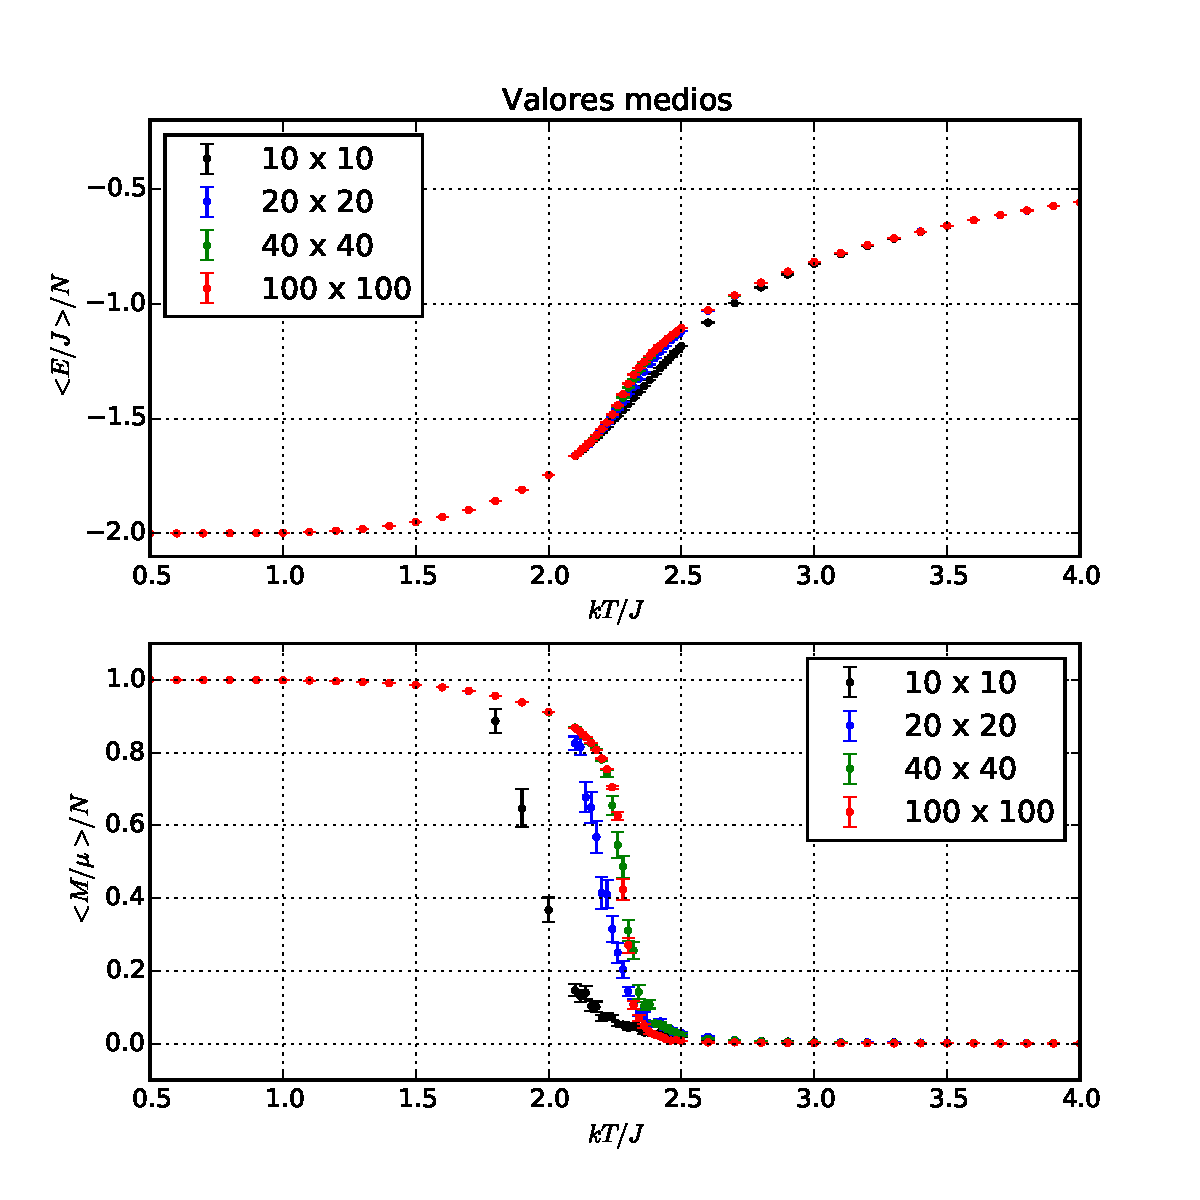
\includegraphics[scale=0.6]{tamano_val_medios.pdf} \\
      \caption{Distribuci�n poissonianas $P(4)$, $P(10)$ y $P(40)$. En rojo 
      aparecen las distribucciones gaussianas para cada 
      caso.}\label{fig:tam_val_medios}
    \end{center}
\end{figure}

\begin{figure}[H]
    \begin{center}
      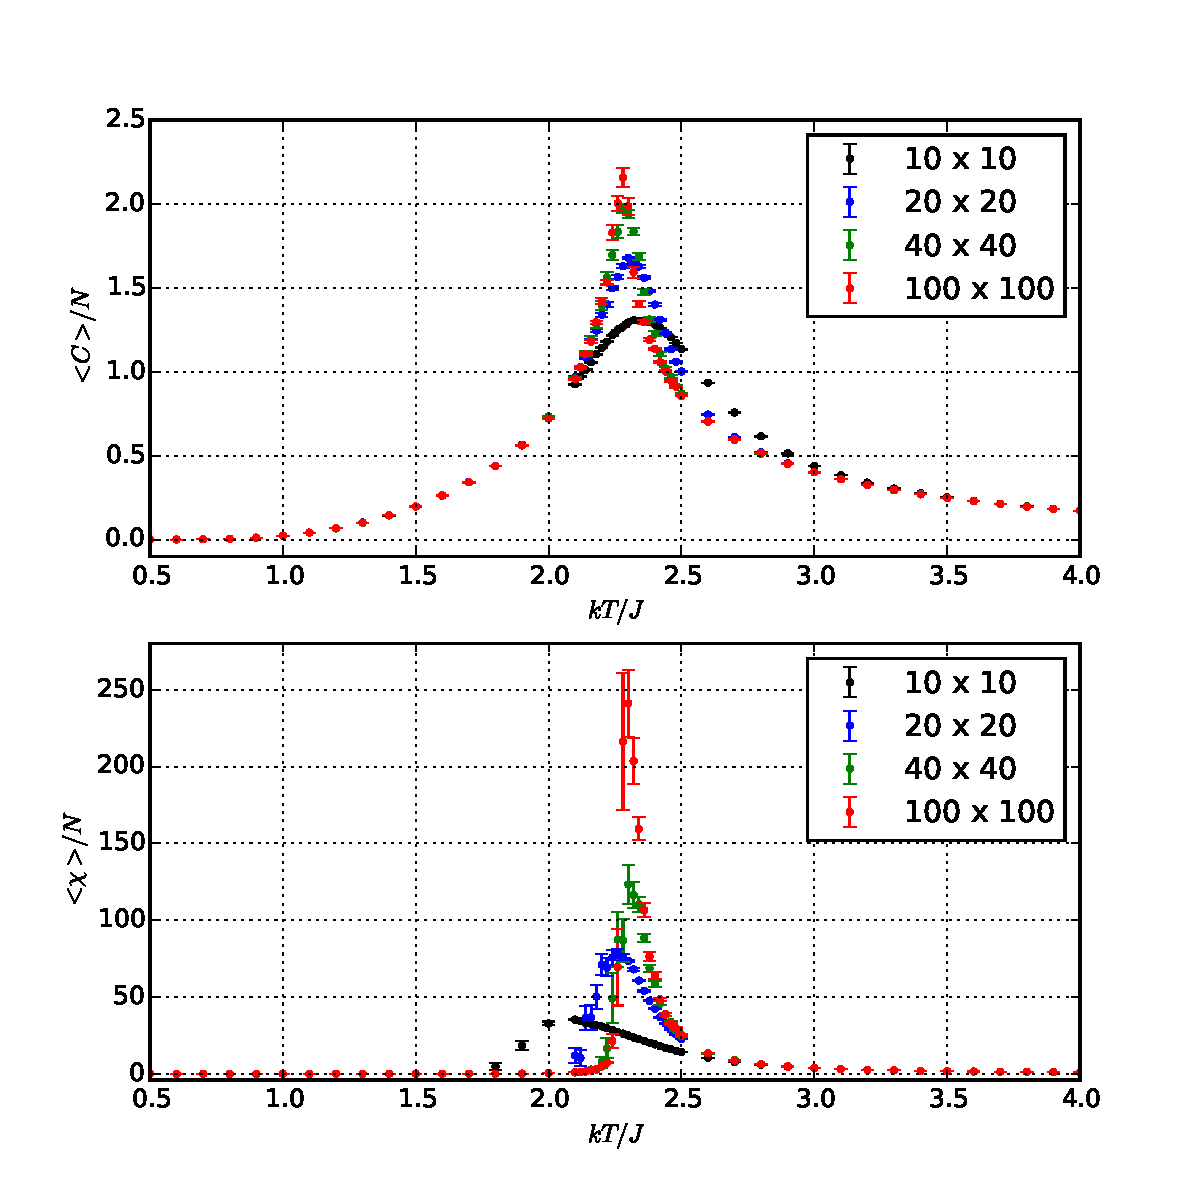
\includegraphics[scale=0.6]{tamano_fluctuaciones.pdf} \\
      \caption{Distribuci�n poissonianas $P(4)$, $P(10)$ y $P(40)$. En rojo 
      aparecen las distribucciones gaussianas para cada 
      caso.}\label{fig:fluctuaciones}
    \end{center}
\end{figure}

\begin{figure}[H]
    \begin{center}
      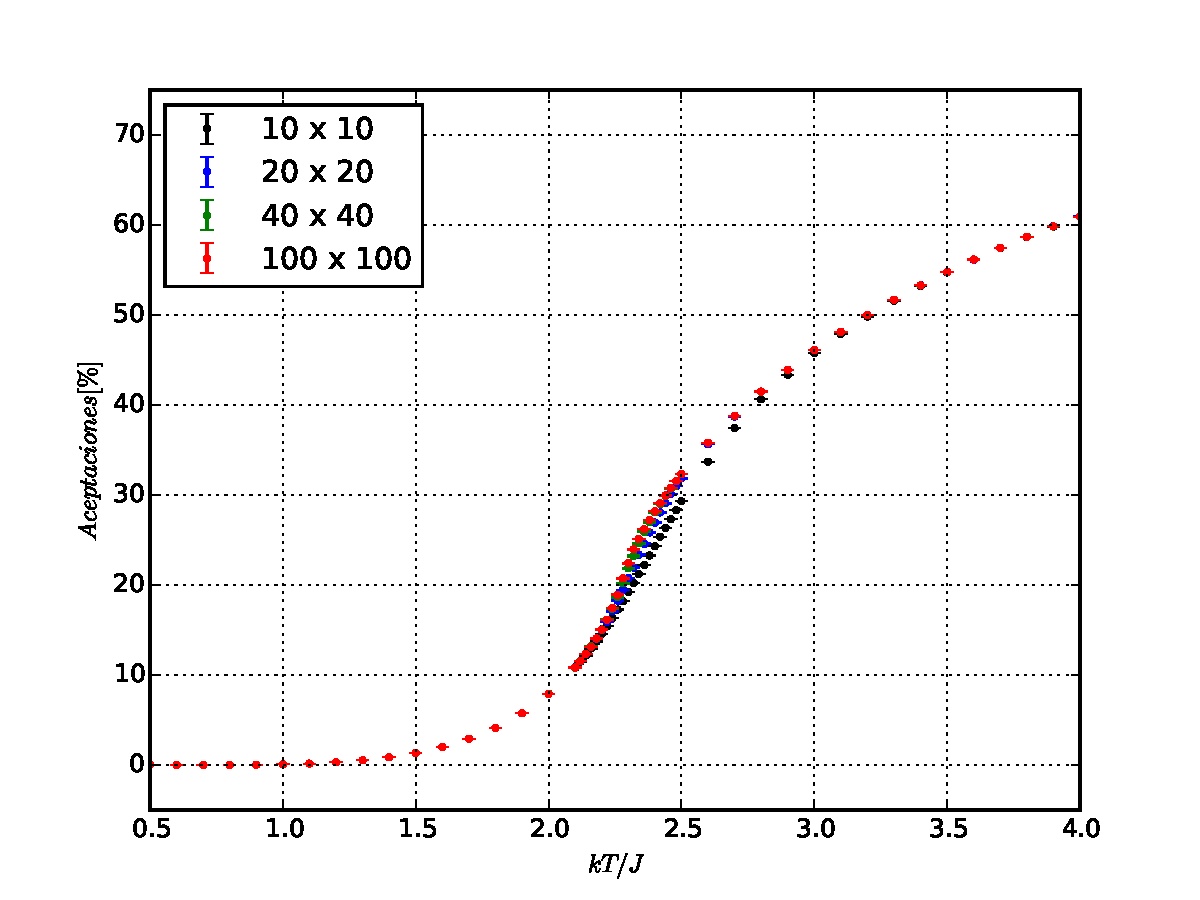
\includegraphics[scale=0.5]{tamano_aceptaciones.pdf} \\
      \caption{Distribuci�n poissonianas $P(4)$, $P(10)$ y $P(40)$. En rojo 
      aparecen las distribucciones gaussianas para cada 
      caso.}\label{fig:aceptaciones}
    \end{center}
\end{figure}

\begin{figure}[H]
    \begin{center}
      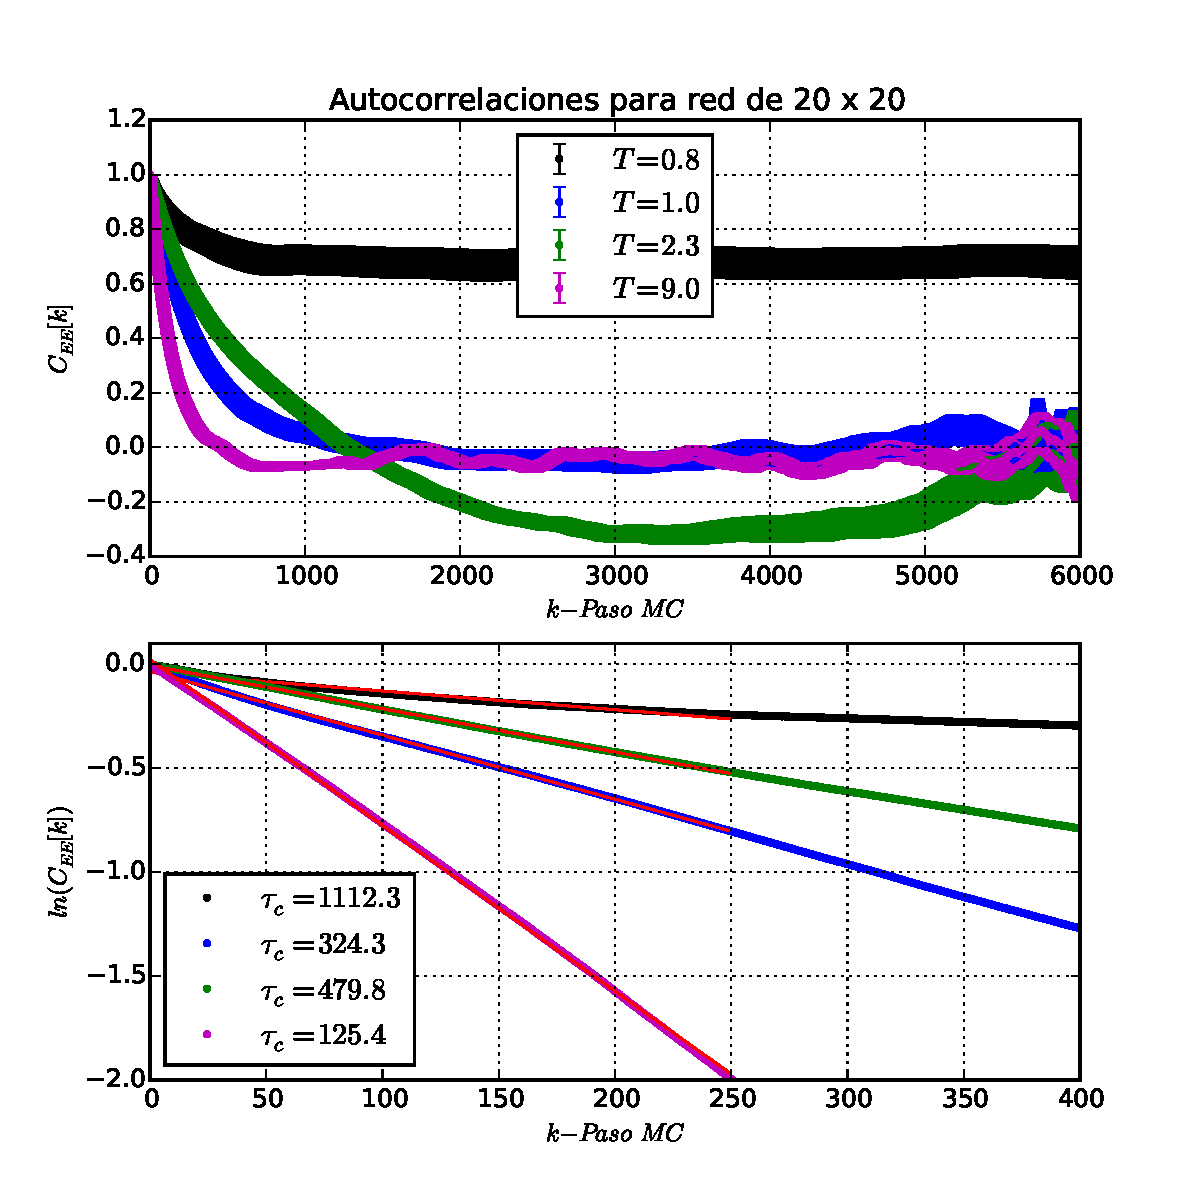
\includegraphics[scale=0.5]{corre_20x20.pdf} \\
      \caption{Distribuci�n poissonianas $P(4)$, $P(10)$ y $P(40)$. En rojo 
      aparecen las distribucciones gaussianas para cada 
      caso.}\label{fig:corre_20x20}
    \end{center}
\end{figure}

\begin{figure}[H]
    \begin{center}
      \includegraphics[scale=0.5]{{corre_tamano_t2.3}.pdf} \\
      \caption{Distribuci�n poissonianas $P(4)$, $P(10)$ y $P(40)$. En rojo 
      aparecen las distribucciones gaussianas para cada 
      caso.}\label{fig:corre_tamano_t2}
    \end{center}
\end{figure}

\begin{figure}[H]
    \begin{center}
      \includegraphics[scale=0.5]{{corre_tamano_t9.0}.pdf} \\
      \caption{Distribuci�n poissonianas $P(4)$, $P(10)$ y $P(40)$. En rojo 
      aparecen las distribucciones gaussianas para cada 
      caso.}\label{fig:corre_tamano_t9}
    \end{center}
\end{figure}

\begin{figure}[H]
    \begin{center}
      \includegraphics[scale=0.5]{{corre_tamano_t9.0}.pdf} \\
      \caption{Distribuci�n poissonianas $P(4)$, $P(10)$ y $P(40)$. En rojo 
      aparecen las distribucciones gaussianas para cada 
      caso.}\label{fig:corre_tamano_t9}
    \end{center}
\end{figure}

%\inputencoding{utf8}
\section {Evoluci\'on de la matriz de estado de spines en funci\'on de la 
temperatura}


Al final de cada ciclo de c\'alculo, en cada una de las  temperaturas, se 
obtiene
la matriz de estado de los spines del sistema.

Un script en python recorre cada una de las carpetas, lee el archivo 
ultimo\_estado.txt,
que graba el programa ising, lo convierte a un array 2D de numpy, para luego 
con la 
librer\'ia matplotlib convertirlo a imagen y grabarlo en disco. 
Luego de grabado en disco con el programa ffmpeg, se obtiene un video que 
muestra
la secuencia de la evoluci\'on del sistema desde temperaturas altas a bajas.



Las figuras \ref{fig:Talta}, \ref{fig:Tmedia},  \ref{fig:Tbaja},  
%\ref{fig:frame2.0},  \ref{fig:frame1.3},  \ref{fig:frame0.5}, 
muestran algunas im\'agenes de esa secuencia correspondientes a  estados
del sistema a temperaturas altas, medias y bajas respectivamente, 
T: 5.0, 3.8, 2.3, 2.0, 1.3 y 0.5.

Al disminuir la temperatura se observa la tendencia a que un valor de spin
tenga m\'as presencia sobre la matriz que el otro. En temperaturas bajas el
spin que mostraba tendencia mayoritaria a temperaturas m\'as altas, termina
siendo el único spin presente en la matriz.




\begin{figure}[H]
	\centering
\begin{subfigure}{.49\textwidth}
	\centering
      \includegraphics[scale=0.3]{{frame5.0}.pdf} \\
      \caption{Temperatura 5.0}\label{fig:frame5.0}
\end{subfigure}
\begin{subfigure}{.49\textwidth}
	\centering
      \includegraphics[scale=0.3]{{frame3.8}.pdf} \\
      \caption{Temperatura 3.8}\label{fig:frame3.8}
\end{subfigure}
      \caption{Temperaturas altas}\label{fig:Talta}
\end{figure}

\begin{figure}[H]
	\centering
\begin{subfigure}{.49\textwidth}
	\centering
      \includegraphics[scale=0.3]{{frame2.3}.pdf} \\
      \caption{Temperatura 2.3}\label{fig:frame2.3}
\end{subfigure}
\begin{subfigure}{.49\textwidth}
	\centering
      \includegraphics[scale=0.3]{{frame2.0}.pdf} \\
      \caption{Temperatura 2.0}\label{fig:frame2.0}
\end{subfigure}

\caption{Temperaturas medias}\label{fig:Tmedia}
\end{figure}

\begin{figure}[H]
	\centering
\begin{subfigure}{.49\textwidth}
	\centering
      \includegraphics[scale=0.3]{{frame1.3}.pdf} \\
      \caption{Temperatura 1.3}\label{fig:frame1.3}
\end{subfigure}
\begin{subfigure}{.49\textwidth}
	\centering
      \includegraphics[scale=0.3]{{frame0.5}.pdf} \\
      \caption{Temperatura 0.5}\label{fig:frame0.5}
\end{subfigure}

\caption{Temperaturas bajas}\label{fig:Tbaja}
\end{figure}

\end{document}
